\documentclass[fleqn,usenatbib]{mnras}

\usepackage{newtxtext,newtxmath}
\usepackage{graphicx}
\usepackage{amsmath}
\usepackage{booktabs}
\usepackage{multirow}
\usepackage{tabularx}
\usepackage{url}
\usepackage{orcidlink}

\title[Calibrating Dyson-sphere selection]{From Dyson-sphere candidates to population constraints: calibrating selection and conditional real-image response in Gaia--2MASS--WISE searches}

\author[Zhang]{
Yuzhan Zhang$^{1}$\orcidlink{0009-0000-3121-7972}\thanks{E-mail: wujijiandao2333@163.com}
\\
$^{1}$Independent Researcher, Beijing, China
}

\date{Accepted XXX. Received YYY; in original form ZZZ}
\pubyear{2026}

\begin{document}
\label{firstpage}
\pagerange{\pageref{firstpage}--\pageref{lastpage}}
\maketitle

\begin{abstract}
Mid-infrared searches for partial Dyson spheres can identify sources consistent with stellar obscuration plus thermal waste heat, but candidate counts cannot be converted into occurrence rates without a selection function matched to the candidate operator. We calibrate several response terms using a 100-pc Gaia DR3 parent sample cross-matched to 2MASS and AllWISE. A 10-band injection--recovery experiment using 265 real stellar templates and a 220,745-model partial-Dyson library yields a conditional SED-recognition response of 0.910 across a 54-cell waste-heat grid. The result is stable to a conservative flux-dependent noise bracket (0.910) and changes to 0.911--0.917 in W2-correction-aware template tests. Combining injected photometric recovery with the \emph{baseline observed} Gaia/WISE host gate on the same 3,000 validation stars gives 0.414 rather than 0.402 from multiplying stage averages; a source-cluster bootstrap gives a 95 per cent interval of 0.0089--0.0147 for the difference. This quantity measures source-level coupling, not counterfactual host completeness. In real AllWISE image injections, leave-one-host-out W3 retention remains unity for 23 baseline-clean hosts under metric/threshold ablations, independent empirical-PSF splits, moderate PSF broadening, and subpixel offsets, giving a one-sided 95 per cent host-level lower bound of 0.878. W4 is qualitatively different: matched-PSF grid-cell retention is unity but falls to 0.451 under mild PSF broadening and 0.362 for a 0.1-pixel injection offset. We therefore treat W4 morphology response as PSF-model dependent. The remaining end-to-end terms are not calibrated, so we do not report a Dyson-sphere occurrence rate.
\end{abstract}

\begin{keywords}
extraterrestrial intelligence -- infrared: stars -- methods: statistical -- catalogues -- surveys
\end{keywords}

\section{Introduction}

The thermodynamic argument that sufficiently large-scale stellar-energy use should generate detectable waste heat has motivated searches for Dyson spheres and related technosignatures for more than six decades \citep{Dyson1960}. Early infrared searches used IRAS to identify approximately blackbody-like sources and place whole-sky upper limits on luminous Dyson spheres \citep{Carrigan2009}. The G-HAT programme subsequently developed a broader formalism for Dysonian searches with WISE and Spitzer, emphasizing both the energy-budget interpretation of mid-infrared emission and the importance of natural dust and source confusion as false positives \citep{Wright2014a,Wright2014b,Griffith2015}. Gaia adds precise distances and optical photometry to this infrared search space, enabling complementary tests based on optical dimming and parallax consistency \citep{Zackrisson2018}.

Project Hephaistos brought these ideas to large stellar samples. Hephaistos-I combined Gaia DR2 and AllWISE to set phenotype-dependent upper limits on partial Dyson spheres \citep{Suazo2022}. Hephaistos-II then developed a Gaia DR3--2MASS--WISE candidate pipeline containing SED fitting, quality cuts, image screening with a convolutional neural network, signal-to-noise requirements, and final visual inspection; seven M-dwarfs survived as candidates for follow-up \citep{Suazo2024}. Subsequent observations have reinforced the importance of the image and contamination terms in such a pipeline. Radio imaging and archival diagnostics indicate background contamination for several systems \citep{Ren2024RNAAS,Ren2025,Ren2026}, while JWST/MIRI resolves background galaxies within approximately one arcsecond of two candidates \citep{Zackrisson2026}. The stellar properties of the broader candidate set remain of astrophysical interest even where an artificial interpretation is disfavoured or unresolved \citep{Korn2026}.

The statistical issue considered here is more general than the status of any individual candidate. A candidate-search pipeline is a measurement operator: a real source must first enter the relevant catalogues, retain usable measurements after the technosignature phenotype modifies its SED, survive deterministic astrophysical and catalogue-quality cuts, remain acceptable in the image domain, and then satisfy the final candidate definition. The rate at which a pipeline produces candidates therefore depends on the underlying population and on the pipeline response.

This perspective is standard in survey astronomy. A selection function is the probability that an object with specified properties enters a scientific sample; importantly, the relevant selection function is unique to the sample actually used for inference \citep{EverallDas2020,BoubertEverall2022}. Gaia provides a particularly clear example: subsets defined by reported astrometry, radial velocity, or RUWE cuts have non-trivial selection functions in magnitude, colour, and position \citep{EverallBoubert2022}. Infrared-excess searches face an additional complication because source confusion can generate apparent excesses: in a WISE study of approximately 180,000 Kepler stars, most nominal warm-dust excesses were attributable to background structure or chance alignments rather than circumstellar emission \citep{KennedyWyatt2012}. These precedents motivate treating a Dyson-sphere candidate list as a selected sample rather than as a direct census of the underlying phenotype.

Let
\begin{equation}
r_{\rm cand}=P({\rm candidate}\mid{\rm star})
\end{equation}
be the candidate rate in a specified stellar parent population,
\begin{equation}
\pi_{\rm DS}=P({\rm DS}\mid{\rm candidate})
\end{equation}
be the fraction of admitted candidates belonging to the target phenotype, and
\begin{equation}
C_{\rm DS}=P({\rm candidate}\mid{\rm DS})
\end{equation}
be the completeness of that same candidate operator for the target phenotype. The common-event identity
\begin{equation}
P({\rm DS}\cap{\rm candidate}\mid{\rm star})
=\pi_{\rm DS}r_{\rm cand}
=f_{\rm DS}C_{\rm DS}
\end{equation}
gives
\begin{equation}
f_{\rm DS}=\frac{\pi_{\rm DS}r_{\rm cand}}{C_{\rm DS}}.
\label{eq:selection_inversion}
\end{equation}
Equation~(\ref{eq:selection_inversion}) is elementary probability, not a new statistical theorem. Its practical force comes from the requirement that all three measured quantities refer to the same parent population, phenotype definition, and candidate-selection operator. A candidate rate measured after a final visual screen cannot consistently be divided by a completeness measured only at an upstream photometric stage.

The purpose of this paper is to calibrate and audit several response terms required by equation~(\ref{eq:selection_inversion}), rather than to claim an occurrence rate. We reconstruct a real 100-pc Gaia DR3 parent sample with 2MASS and AllWISE cross-matches, perform partial-Dyson injection--recovery on real stellar SEDs, combine the injected photometric response with the \emph{baseline observed} Gaia/WISE host-quality state of the same sources, and then test co-spatial waste-heat injection in real AllWISE W3/W4 images. The image experiment is leave-one-host-out, so a tested star contributes neither to the empirical PSF used to inject it nor to the empirical morphology calibration used to classify it. We additionally challenge the image operator by separating or perturbing the injection PSF from the scoring PSF, and we audit photometric saturation and flux-dependent noise assumptions. This approach isolates which pieces of the response are currently measured and which remain external-validity limitations.

The contribution is therefore operational rather than a claim to have invented selection-function theory. We make three empirical advances specific to partial-Dyson searches: (i) we measure the same-source coupling between injected photometric recovery and an observed baseline host-quality gate, exposing the bias in multiplying stage-average efficiencies while explicitly separating this quantity from full counterfactual host completeness; (ii) we move the image-response experiment from a Gaussian image emulator to real AllWISE intensity, uncertainty, and coverage data with epoch-corrected source positions and leave-one-host-out calibration, then stress-test PSF-model dependence; and (iii) we separate field-environment rejection, bright-source non-linearity, and conditional morphology response so that these distinct effects are not compressed into a single ``image completeness'' number. The inferential contribution is to connect measured response terms to a selection-consistent candidate-to-population inversion while leaving unmeasured terms explicit.

\section{Data, parent sample, and conditioning structure}
\label{sec:data}

\subsection{Gaia DR3 mother sample and cross-matches}

We selected Gaia DR3 sources with parallax greater than 10 mas, corresponding nominally to distances smaller than 100 pc. The resulting mother catalogue contains 574,531 Gaia sources. We intentionally did not pre-clean this catalogue by RUWE, signal-to-noise ratio, or astrophysical-parameter availability: removing problematic sources before defining the response would turn part of the selection process into an undocumented precondition.

The Gaia mother sample was cross-matched separately to 2MASS \citep{Skrutskie2006} and AllWISE \citep{Wright2010,Cutri2013}. Cross-match results were merged locally with left joins so that missing counterparts remained explicit. In the full mother sample, 47.49 per cent have an AllWISE counterpart and 52.36 per cent have a 2MASS counterpart. These raw fractions are not interpreted as Dyson-sphere completeness; the mother catalogue intentionally contains a broad set of Gaia sources that are not all suitable for a ten-band stellar SED analysis.

\subsection{Main-sequence selection}

We defined a broad colour--magnitude main-sequence sample in absolute Gaia $G$ magnitude and $G_{\rm BP}-G_{\rm RP}$ colour. A source is rejected as a giant when
\begin{equation}
M_G<4
\quad\hbox{and}\quad
M_G<7(G_{\rm BP}-G_{\rm RP})-3,
\end{equation}
and rejected as a white-dwarf/high-absolute-magnitude source when
\begin{equation}
M_G>3(G_{\rm BP}-G_{\rm RP})+5.
\end{equation}
We additionally retain $0\le M_G\le13.6$. This produces 250,909 candidate main-sequence stars; 204,613 of them have RUWE $<1.4$. Figure~\ref{fig:cmd} shows the selection.

\begin{figure}
\centering
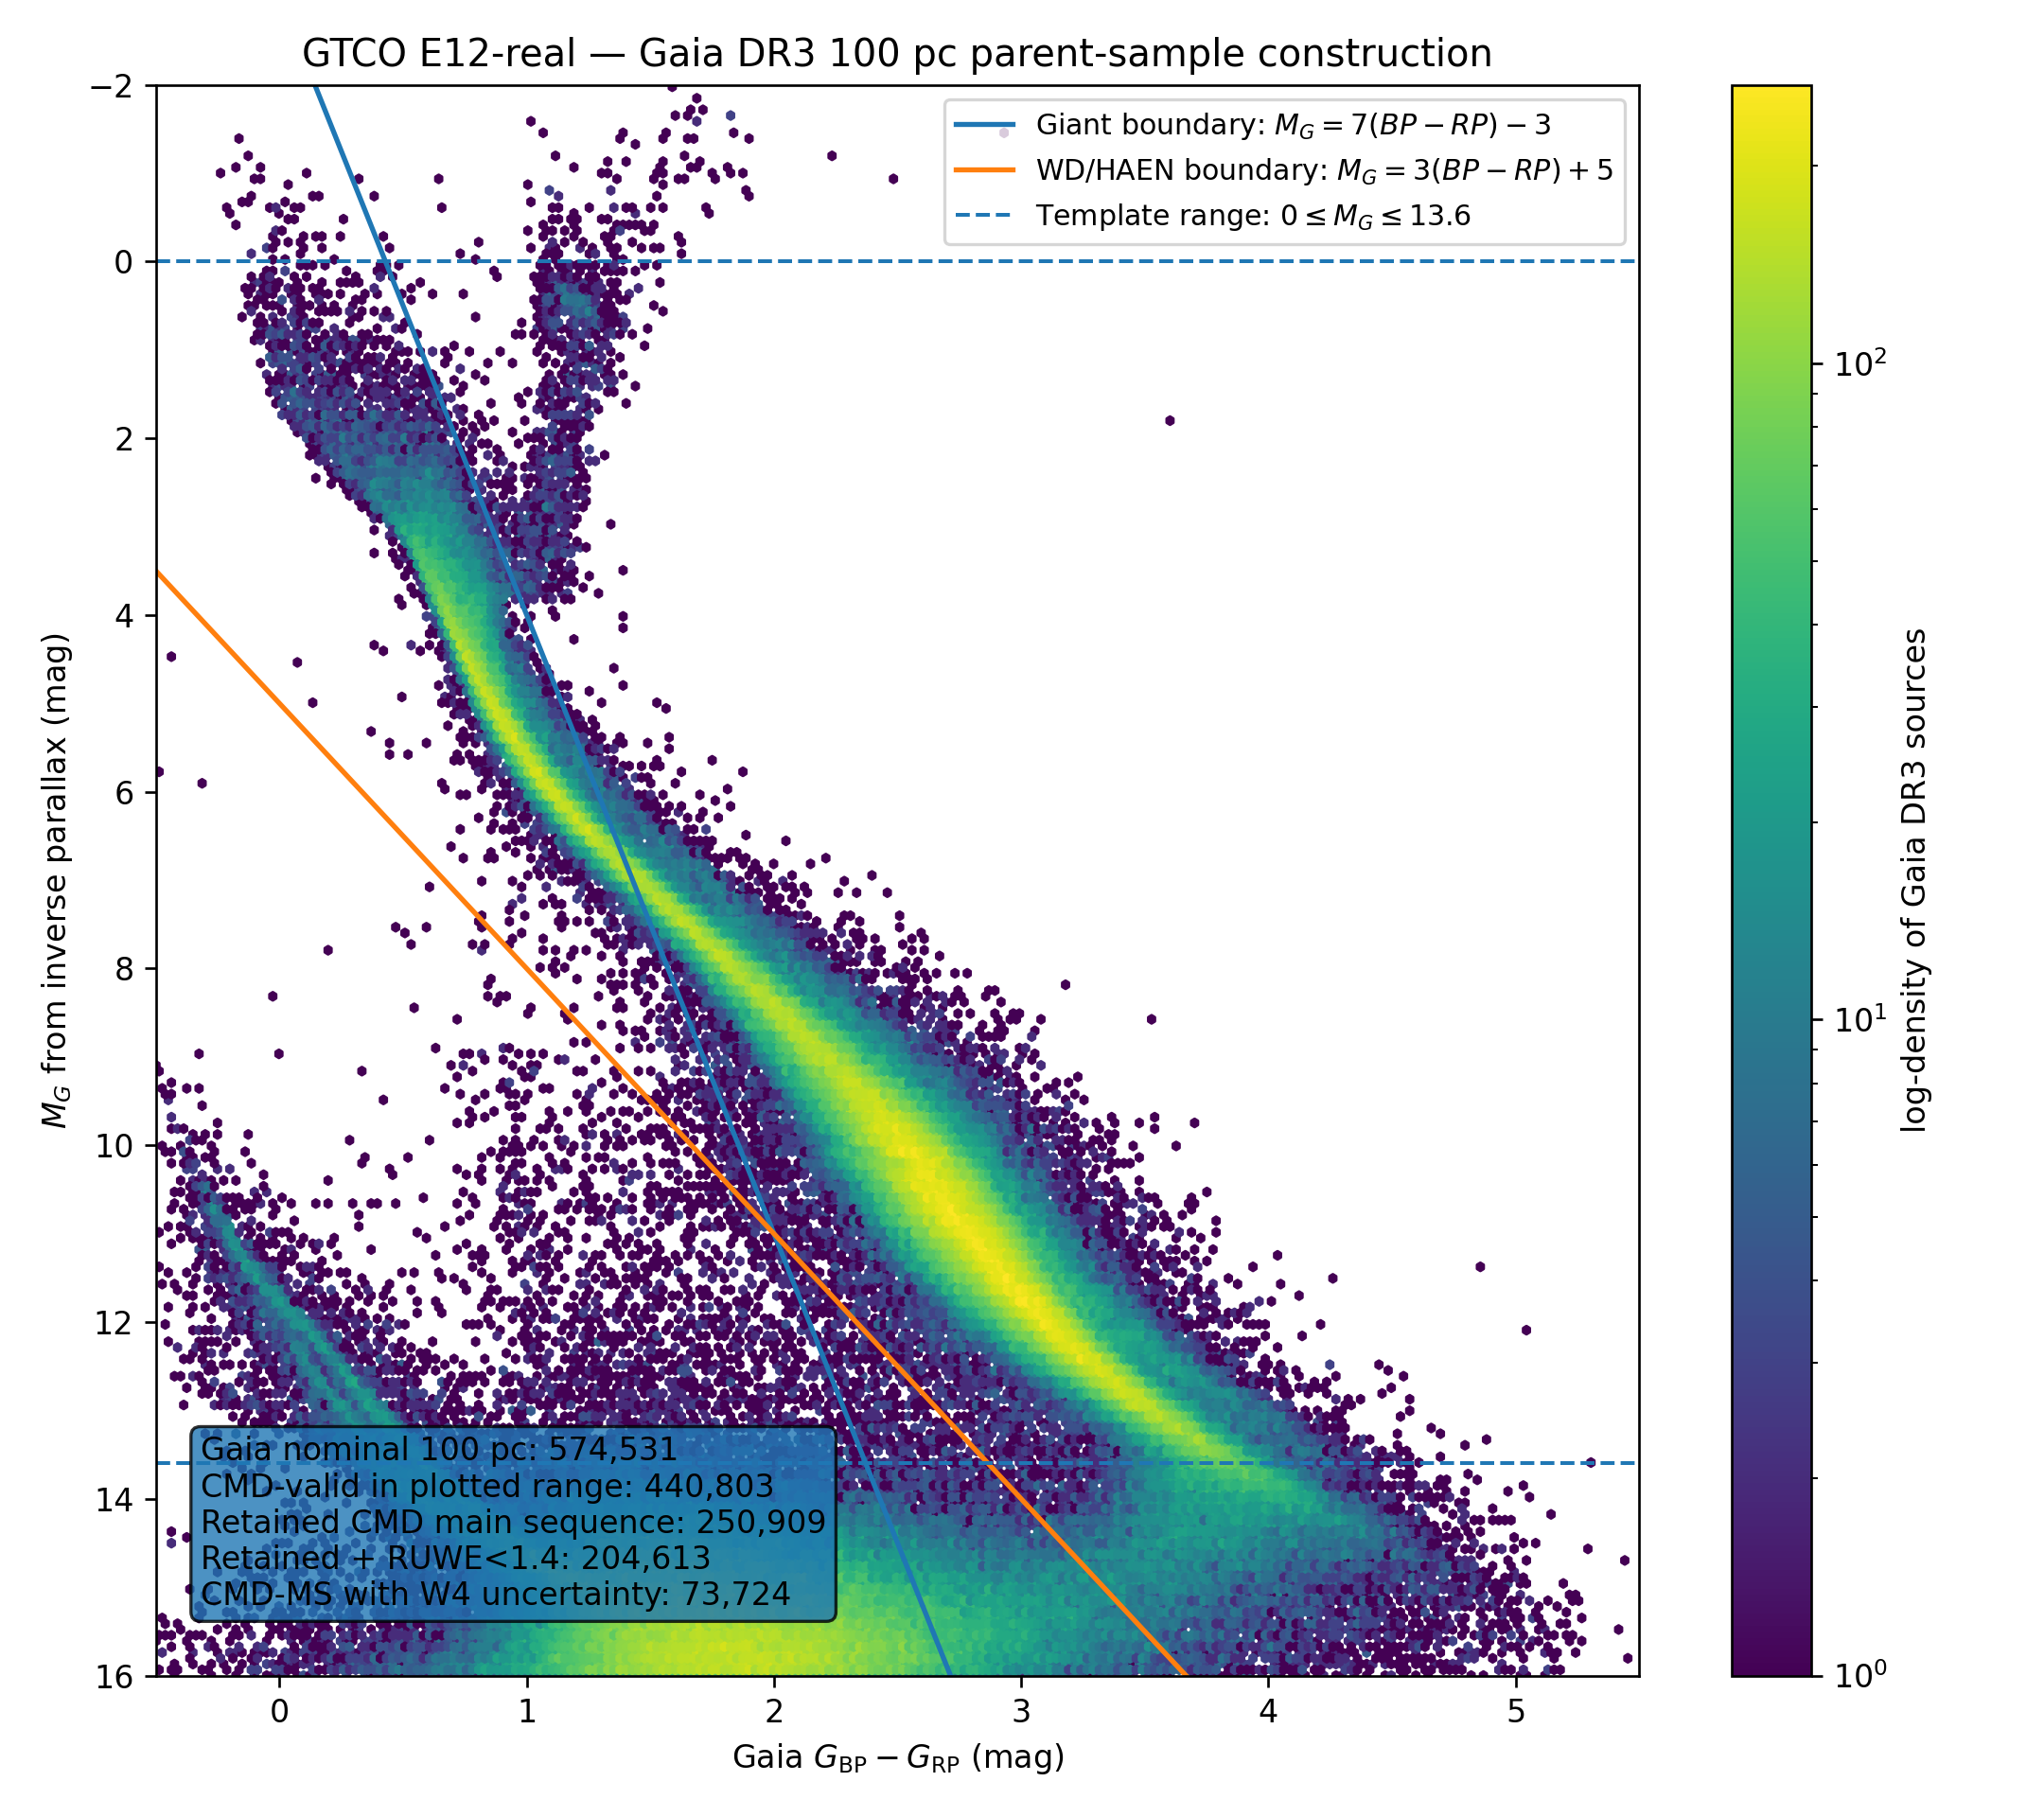
\includegraphics[width=\columnwidth]{figures/fig1_cmd.png}
\caption{Gaia DR3 colour--magnitude selection for the nominal 100-pc parent sample. Downstream host-quality cuts are intentionally not incorporated into this boundary, so their response remains measurable.}
\label{fig:cmd}
\end{figure}

\subsection{Conditioning matters}
\label{sec:conditioning}

The injection experiment described below is not performed on every one of the 250,909 main-sequence stars. It uses a validation-eligible subset with complete baseline photometry and uncertainties. In the real catalogue, 72,716 of the 250,909 CMD-selected stars (28.98 per cent) satisfy the strict ten-band-with-errors requirement used to construct the clean template/validation pool. This fraction is reported to make the conditioning explicit; it is not multiplied into our quoted 0.910 photometric recovery because the strict validation-pool definition is an engineering requirement of the present emulation, not a reconstruction of every admission rule in Hephaistos-II.

We therefore distinguish three different quantities throughout the paper:
\begin{enumerate}
\item a \emph{parent-sample availability} problem, which asks which real stars provide the information needed by a particular analysis;
\item a \emph{conditional injection response}, which asks how a counterfactual Dyson-like source propagates after a usable baseline SED has been established; and
\item an \emph{end-to-end candidate completeness}, which would require all published pipeline stages to be represented by the same executable operator.
\end{enumerate}
Only the second is directly calibrated by the 0.910 recovery reported in Section~\ref{sec:phot}. Table~\ref{tab:semantic} summarizes this distinction.

\begin{table*}
\centering
\caption{Selection terms and their interpretation in this work. ``Measured'' means measured for the stated conditioning set, not necessarily for the full 300-pc Hephaistos-II parent population.}
\label{tab:semantic}
\begin{tabularx}{\textwidth}{p{0.16\textwidth} X p{0.17\textwidth} p{0.25\textwidth}}
\toprule
Term & Operational meaning & Current status & Principal conditioning / limitation\\
\midrule
Baseline catalogue availability & Required real measurements exist & Described, not inverted & Analysis-specific ten-band validation pool\\
$C_{\rm phot\mid V}$ & Injected source survives proxy catalogue cuts and is SED-recognised & Measured & Conditional on validation-eligible hosts $V$\\
$C_{\rm host\mid V}$ & Same validation host passes deterministic Gaia/WISE cuts & Measured & Reconstructed subset of published host cuts\\
$C_{\rm phot\cap host\mid V}$ & Same injected source passes both previous terms & Measured source-by-source & Does not include original CNN/final visual screen\\
$R_{\rm morph}$ & True co-spatial excess remains morphology-acceptable & Measured conditionally & 24 deliberately clean real WISE fields; unsaturated regime\\
$C_{\rm environment}$ & Real field is acceptable before signal injection & Not yet population-calibrated & Requires representative crowded/background sample\\
$C_{\rm linear}$ & Counterfactual remains in usable detector/catalogue regime & Risk surface measured & Saturated images not forward-modelled\\
$C_{\rm DS}$ & Full candidate-operator response & Not yet measured & Requires all stages with matched candidate definition\\
\bottomrule
\end{tabularx}
\end{table*}

\section{Photometric partial-Dyson injection--recovery}
\label{sec:phot}

\subsection{Phenotype model}

We parameterize a partial Dyson sphere by a covering factor $\gamma$ and a waste-heat temperature $T_{\rm DS}$. In the energy-conserving single-temperature model used for the injection library, the observed stellar component is attenuated by $1-\gamma$, while a fraction $\gamma$ of the stellar bolometric flux is thermally re-radiated. The monochromatic model flux density is
\begin{equation}
F_{\nu,{\rm model}}=(1-\gamma)F_{\nu,\star}
+\gamma F_{{\rm bol},\star}
\frac{\pi B_\nu(T_{\rm DS})}{\sigma_{\rm SB}T_{\rm DS}^4}.
\label{eq:dsmodel}
\end{equation}
This is a search phenotype rather than a claim that real technospheres must be blackbodies. The same physical distinction applies to previous Dysonian searches: detectability statements are conditional on the waste-heat phenotype being searched \citep{Wright2014b,Suazo2022}. Our implementation evaluates the model at the adopted band reference wavelengths rather than performing a new full response-curve integration; this and the exact template library are among the reasons we describe the experiment as a close emulation rather than a byte-for-byte reconstruction of Hephaistos-II.

\subsection{Real stellar templates}

The model library is anchored to 265 real stars from the downloaded 100-pc catalogue, mirroring the published number of stellar templates in Hephaistos-II \citep{Suazo2024}. Candidate templates must lie on the CMD main sequence, have RUWE $<1.4$, have all ten magnitudes and the required uncertainty information, satisfy AllWISE ${\tt cc\_flags}=0000$ and ${\tt ext\_flag}=0$, and have a star-only near/mid-infrared baseline residual below 0.2 mag. The final 265 are selected to span the available $M_G$ sequence rather than being a random draw concentrated near the peak of the luminosity function.

Each template is transformed to absolute photometry at 10 pc. For Gaia $G$, $G_{\rm BP}$, and $G_{\rm RP}$, the stellar flux is grey-attenuated by $1-\gamma$. For 2MASS $JHK_s$ and WISE W1--W4, equation~(\ref{eq:dsmodel}) supplies the sum of attenuated stellar light and thermal waste heat. We combine the 265 templates with 49 temperatures between 100 and 700 K and 17 covering factors between 0.1 and 0.9, producing
\begin{equation}
265\times49\times17=220,745
\end{equation}
model SEDs. The published Hephaistos-II description provides the ranges and model counts; because the exact internal grid spacing was not available to this reconstruction, we use uniform grids within those ranges.

\subsection{Independent validation stars and noise model}

A separate set of 3,000 real main-sequence stars is excluded from the 265-template library and used for validation. These stars have all ten bands and their required errors available, baseline stellar-model residual below 0.2 mag, and a conservative star-only mid-infrared residual proxy below 0.5 mag. The validation stars are sampled across the sorted $M_G$ sequence to maintain broad coverage of the selected main sequence rather than selecting 3,000 adjacent objects in luminosity.

The truth grid contains nine waste-heat temperatures,
\begin{equation}
T_{\rm DS}=\{100,150,200,250,300,400,500,600,700\}\ {\rm K},
\end{equation}
and six covering factors,
\begin{equation}
\gamma=\{0.1,0.2,0.3,0.5,0.7,0.9\},
\end{equation}
for 54 truth cells. For each source, the counterfactual flux is perturbed using that source's measured per-band photometric uncertainty in flux space. The noisy ten-band SED is transformed to absolute magnitudes and queried against the 220,745-model library by Euclidean nearest-neighbour distance. Following the unweighted magnitude-space criterion described for Hephaistos-II, the recognition statistic is
\begin{equation}
{\rm RMSE}=\frac{d_{10}}{\sqrt{10}},
\end{equation}
with acceptance at RMSE $\le0.2$ mag \citep{Suazo2024}. The use of an unweighted magnitude RMSE prevents the highest signal-to-noise optical bands from automatically dominating the W3/W4 excess geometry, but it is also a deliberate model choice and is not interpreted as a likelihood.

\subsection{Catalogue-survival proxy and saturation flag}

Before model recognition, an injected source must retain positive noisy flux in all ten bands, have injected Gaia $G\le21$, have expected 2MASS $JHK_s$ signal-to-noise ratio $>2$, and have expected W3/W4 signal-to-noise ratio $>3.5$. These cuts are a reconstruction of the relevant photometric stage, not the complete Hephaistos-II candidate operator. WISE saturation risk is tracked separately. We use the WISE characteristic point-source saturation magnitudes W3 $=3.8$ and W4 $=-0.4$ mag, at which approximately half of catalogue sources show saturation; saturated-source photometry can remain recoverable from unsaturated wings, but its accuracy becomes progressively less reliable \citep{Cutri2012}.

Across the 54 truth cells, the mean catalogue-survival proxy is 0.9863. Conditional on catalogue survival, the mean model-recognition probability is 0.9206. Counting both survival and recognition, the arithmetic mean over the 54 equally weighted truth cells is
\begin{equation}
\left\langle C_{\rm phot\mid V}\right\rangle=0.9101.
\end{equation}
This is a grid average, not a population-marginalized completeness: changing the phenotype distribution over $(T_{\rm DS},\gamma)$ would change the average. Figure~\ref{fig:photrec} shows the response surface. The weakest cell is the cold, high-covering-factor region, where catalogue survival, finite-band contrast, and saturation become most consequential.

\begin{figure}
\centering
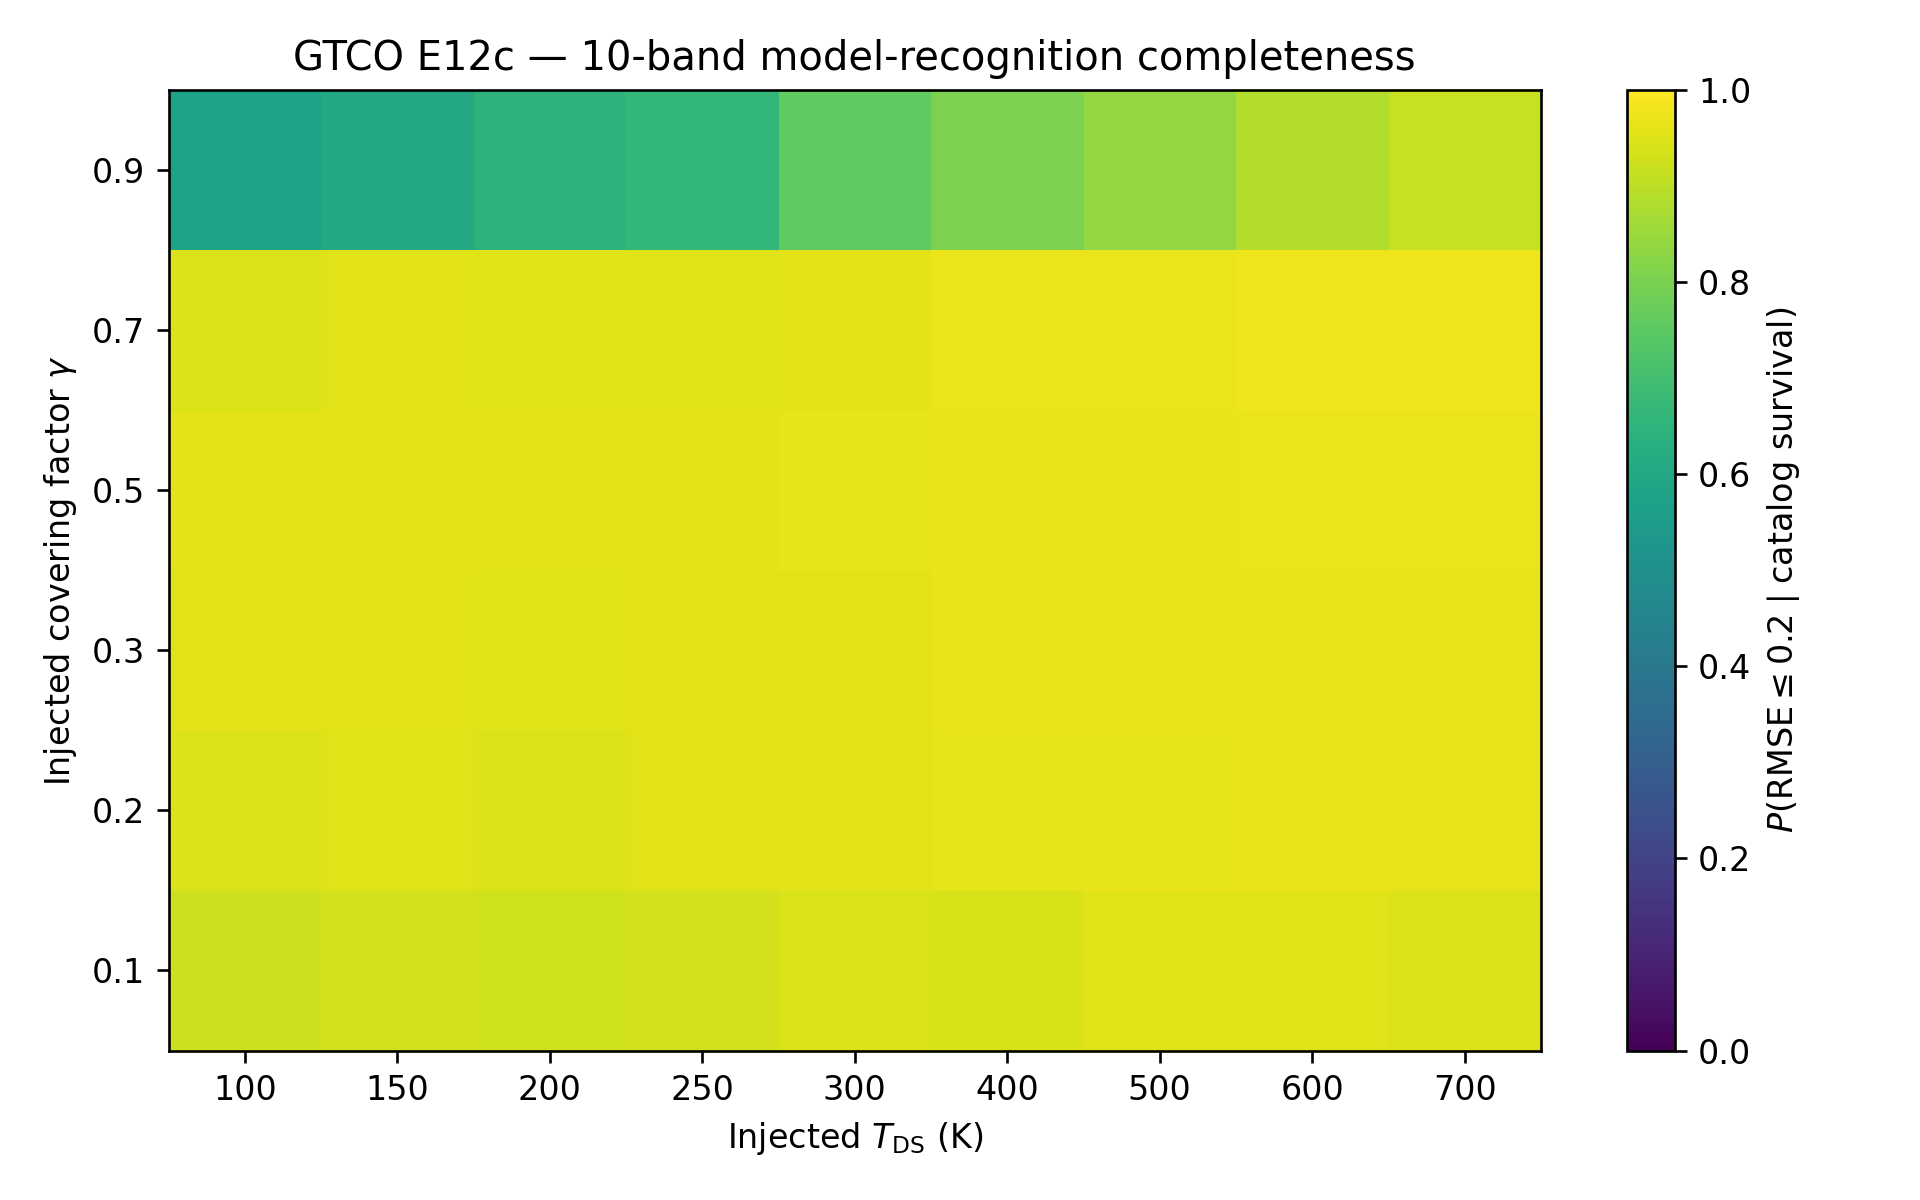
\includegraphics[width=\columnwidth]{figures/fig2_photometric_recovery.png}
\caption{Real-catalogue injection--recovery across the 54-cell partial-Dyson truth grid. The response includes the stated catalogue-survival proxy and ten-band model recognition, conditional on the validation-eligible real stellar sample. It is not the end-to-end candidate completeness.}
\label{fig:photrec}
\end{figure}

\subsection{WISE-template saturation and photometric-noise sensitivity}
\label{sec:phot_robustness}

The published Hephaistos-II template-selection appendix states that WISE saturation limits of W1 $=8.1$, W2 $=6.7$, W3 $=3.8$, and W4 $=-0.4$ mag were considered, and that a W2 correction following \citet{CottenSong2016} was applied \citep{Suazo2024}. Our frozen 265-star emulation does not reproduce the original template identities: 86/265 frozen templates are brighter than 8.1 mag in W1 and 58/265 are brighter than 6.7 mag in W2, while none cross the W3 or W4 characteristic thresholds. We therefore do not describe the frozen library as an exact reproduction of the original saturation semantics.

The separate 3,000-star validation set is not restricted by the template-star saturation rule: 51.4 per cent and 14.5 per cent of its baseline rows are brighter than the W1 and W2 nominal saturation onsets, respectively, while only 0.1 per cent cross the W3 onset and none cross the W4 onset. As an additional conditioning check, restricting validation to the 1,458 stars fainter than all four nominal WISE saturation onsets increases the mean recovery to 0.947213. Because this restriction changes the luminosity and host distribution of the validation population, we report it as a subset sensitivity rather than treating it as a correction to the baseline 0.9105 response.

We performed two correction-aware sensitivity tests. Applying the W2 correction while retaining the frozen template identities changes the mean response from 0.910537 to 0.911086. Reselecting a 265-star template sequence with the correction applied while preserving the bright-to-faint $M_G$ coverage gives 0.916605. By contrast, interpreting all four quoted WISE saturation-onset magnitudes as literal hard exclusion cuts removes the bright end of the available template sequence ($M_G$ then begins near 4.46 rather than near 0) and gives 0.696488. Because this literal hard-cut construction no longer reproduces the published broad $M_G$ template coverage, we retain it only as a deliberately severe stress test rather than as the preferred emulation. WISE documentation likewise distinguishes the onset of saturation from complete loss of measurable source flux, since some saturated-source photometry can be recovered from PSF wings \citep{Cutri2012}.

WISE broad-band response is a separate concern from W2 saturation correction. The WISE photometric calibration explicitly requires spectral colour corrections for steep mid-infrared spectra, especially in the broad W3 passband \citep{Wright2010}. For example, the tabulated 100-K blackbody factor is $f_c({\rm W3})=2.6588$. We therefore repeated the full library construction and 54-cell recovery after applying the published blackbody colour-correction factors to the added waste-heat component in W1--W4, using log-temperature interpolation between the tabulated 100, 141, 200, 283, 400, 566, and 800-K anchors. Retaining the frozen reference wavelengths gives a mean recovery of 0.912309. Replacing the WISE reference wavelengths by the published isophotal values (3.3526, 4.6028, 11.5608, and 22.0883~$\mu$m) while applying the same colour corrections gives 0.911568. Thus, even though the coldest W3 correction is individually large, incorporating the WISE broad-band response at this level changes the equally weighted grid-average response by only $1$--$2\times10^{-3}$. This is a sensitivity calculation using the published WISE colour-correction system, not a claim of exact full-pipeline synthetic photometry.

The baseline injection also keeps each source's measured absolute flux uncertainty fixed as the counterfactual flux changes. To test the sensitivity of the 0.91 result to that approximation, we bracketed alternative flux-dependent noise laws. A conservative floor-plus-Poisson model,
\begin{equation}
\sigma_{F,\rm cf}=\sigma_{F,0}\sqrt{\max(1,F_{\rm cf}/F_0)},
\end{equation}
prevents artificially improved absolute noise when a source is dimmed while allowing Poisson-like growth for brighter counterfactuals. It yields a mean recovery of 0.910309, only $2.3\times10^{-4}$ below the frozen baseline. More extreme pure-Poisson and constant-fractional prescriptions give 0.955685 and 0.701735, respectively; we treat these as sensitivity brackets rather than detector models. Table~\ref{tab:photrobust} summarizes the tests.

\begin{table}
\centering
\caption{Photometric robustness tests. The WISE blackbody colour-correction row applies the published W1--W4 blackbody response factors and WISE isophotal wavelengths. The hard four-band saturation-onset cut is a deliberately severe stress test because it eliminates the bright end of the template sequence; it is not the preferred reconstruction.}
\label{tab:photrobust}
\begin{tabular}{lr}
\toprule
Variant & Mean recovery\\
\midrule
Frozen baseline & 0.910537\\
Frozen templates + W2 correction & 0.911086\\
Correction-aware template sequence & 0.916605\\
WISE BB colour corr. + isophotal $\lambda$ & 0.911568\\
Conservative floor+Poisson noise & 0.910309\\
Hard four-band onset cut (stress) & 0.696488\\
\bottomrule
\end{tabular}
\end{table}

\subsection{Independent reconstruction audit}

The submission-grade standalone reconstruction rebuilds the 220,745-model library from the frozen 265 real templates and reruns all 54 truth cells on the 3,000 validation stars without reading frozen summary tables as inputs. It gives mean catalogue survival 0.986302 and mean photometric recovery 0.910537, compared with frozen references 0.986309 and 0.910543. The absolute differences are $6.2\times10^{-6}$ in both headline quantities. This executable reconstruction is used for the same-source host-coupling analysis below.

\section{Deterministic host selection}
\label{sec:hostcuts}

\subsection{Gaia/WISE fields and operational cuts}

Hephaistos-II applies astrophysical and catalogue-quality filters intended to reduce stellar activity, variability, astrometric complexity, source extension, and non-stellar contamination \citep{Suazo2024}. We downloaded the Gaia DR3 quantities needed to reconstruct the available cuts, including H$\alpha$ equivalent width and uncertainty, $G$-band observation counts and flux-over-error, and the DSC combined probability of being a single star. Gaia DR3 Apsis provides the H$\alpha$ and classification products used here \citep{Creevey2023}. RUWE is the Gaia renormalised astrometric goodness-of-fit statistic \citep{Lindegren2021}; it is itself known to define a non-trivial Gaia subset selection \citep{EverallBoubert2022}.

Our operational host gate requires
\begin{align}
EW_{{\rm H}\alpha}+3\sigma_{EW}&\ge0,\\
G_{\rm var}&\le2,\\
{\rm RUWE}&\le1.4,\\
{\tt ext\_flag}&=0,\\
P_{\rm Gaia,star}&>0.9.
\end{align}
The H$\alpha$ condition rejects a source only when the measured equivalent width plus three standard deviations remains on the emission side of the adopted sign convention. Missing H$\alpha$ does not by itself constitute evidence for emission and therefore does not trigger this rejection. In contrast, missing RUWE, WISE extension flag, stellar-classification probability, or variability statistic cannot satisfy their positive quality requirements and are treated as failures of those individual cuts. These semantics are frozen in the public reproduction script.

\subsection{Variability statistic and sensitivity to the reference window}

We reconstruct the reported $G$-band variability statistic from
\begin{equation}
\nu_G=\frac{\sqrt{N_{{\rm obs},G}}}
{{\tt phot\_g\_mean\_flux\_over\_error}},
\end{equation}
and normalize it by a local median among sources of similar $G$ magnitude,
\begin{equation}
G_{\rm var}=\frac{\nu_G}
{\operatorname{median}_{\rm similar\,G}(\nu_G)}.
\end{equation}
The published description does not uniquely specify the numerical width of the ``similar-flux'' neighbourhood. We therefore evaluated rolling reference windows of 500, 1,000, and 5,000 magnitude-sorted sources. In the 250,909-star CMD main-sequence sample, the full host-pass fractions are 0.522819, 0.522875, and 0.522994, respectively. Pairwise classification disagreement is below 0.4 per cent. We adopt 1,000 as the default while carrying the window sensitivity as an audit rather than presenting the choice as known exactly.

\subsection{Baseline observed host gate in the injection validation sample}

The deterministic gate is evaluated on the \emph{observed baseline catalogue row} of each of the same 3,000 validation stars. Sequential retention is 0.925 after H$\alpha$, 0.760 after adding $G_{\rm var}$, 0.572 after RUWE, 0.526 after AllWISE extension, and
\begin{equation}
C_{\rm host,base\mid V}=0.442
\end{equation}
after the stellar-classification requirement.

This quantity is intentionally labelled a \emph{baseline} host gate. The injected partial-Dyson SED changes the apparent stellar flux, and a sufficiently large $\gamma$ could alter Gaia signal-to-noise, classification availability, or the distribution of quality statistics. The present experiment does not forward-model those catalogue products under the counterfactual source. We tested an exploratory nearest-neighbour model for counterfactual host response in the parent catalogue, but dimmed injected sources move away from the ordinary main-sequence training manifold; we therefore do not promote that extrapolative model into the headline analysis. A full $P({\rm host\ pass}\mid{\rm DS})$ remains an uncalibrated term.

Because the five baseline cuts overlap, the marginal number removed by a cut depends on its order. We therefore calculated a Shapley attribution over all $5!=120$ cut orderings. RUWE accounts for 38.9 per cent of the attributed baseline host-selection loss, followed by $G_{\rm var}$ (20.6 per cent), stellar-classification probability (20.3 per cent), WISE extension (11.6 per cent), and H$\alpha$ (8.6 per cent; Fig.~\ref{fig:shapley}). This is a decomposition of selection burden, not an argument that the largest-contribution cut is astrophysically unjustified.

\begin{figure}
\centering
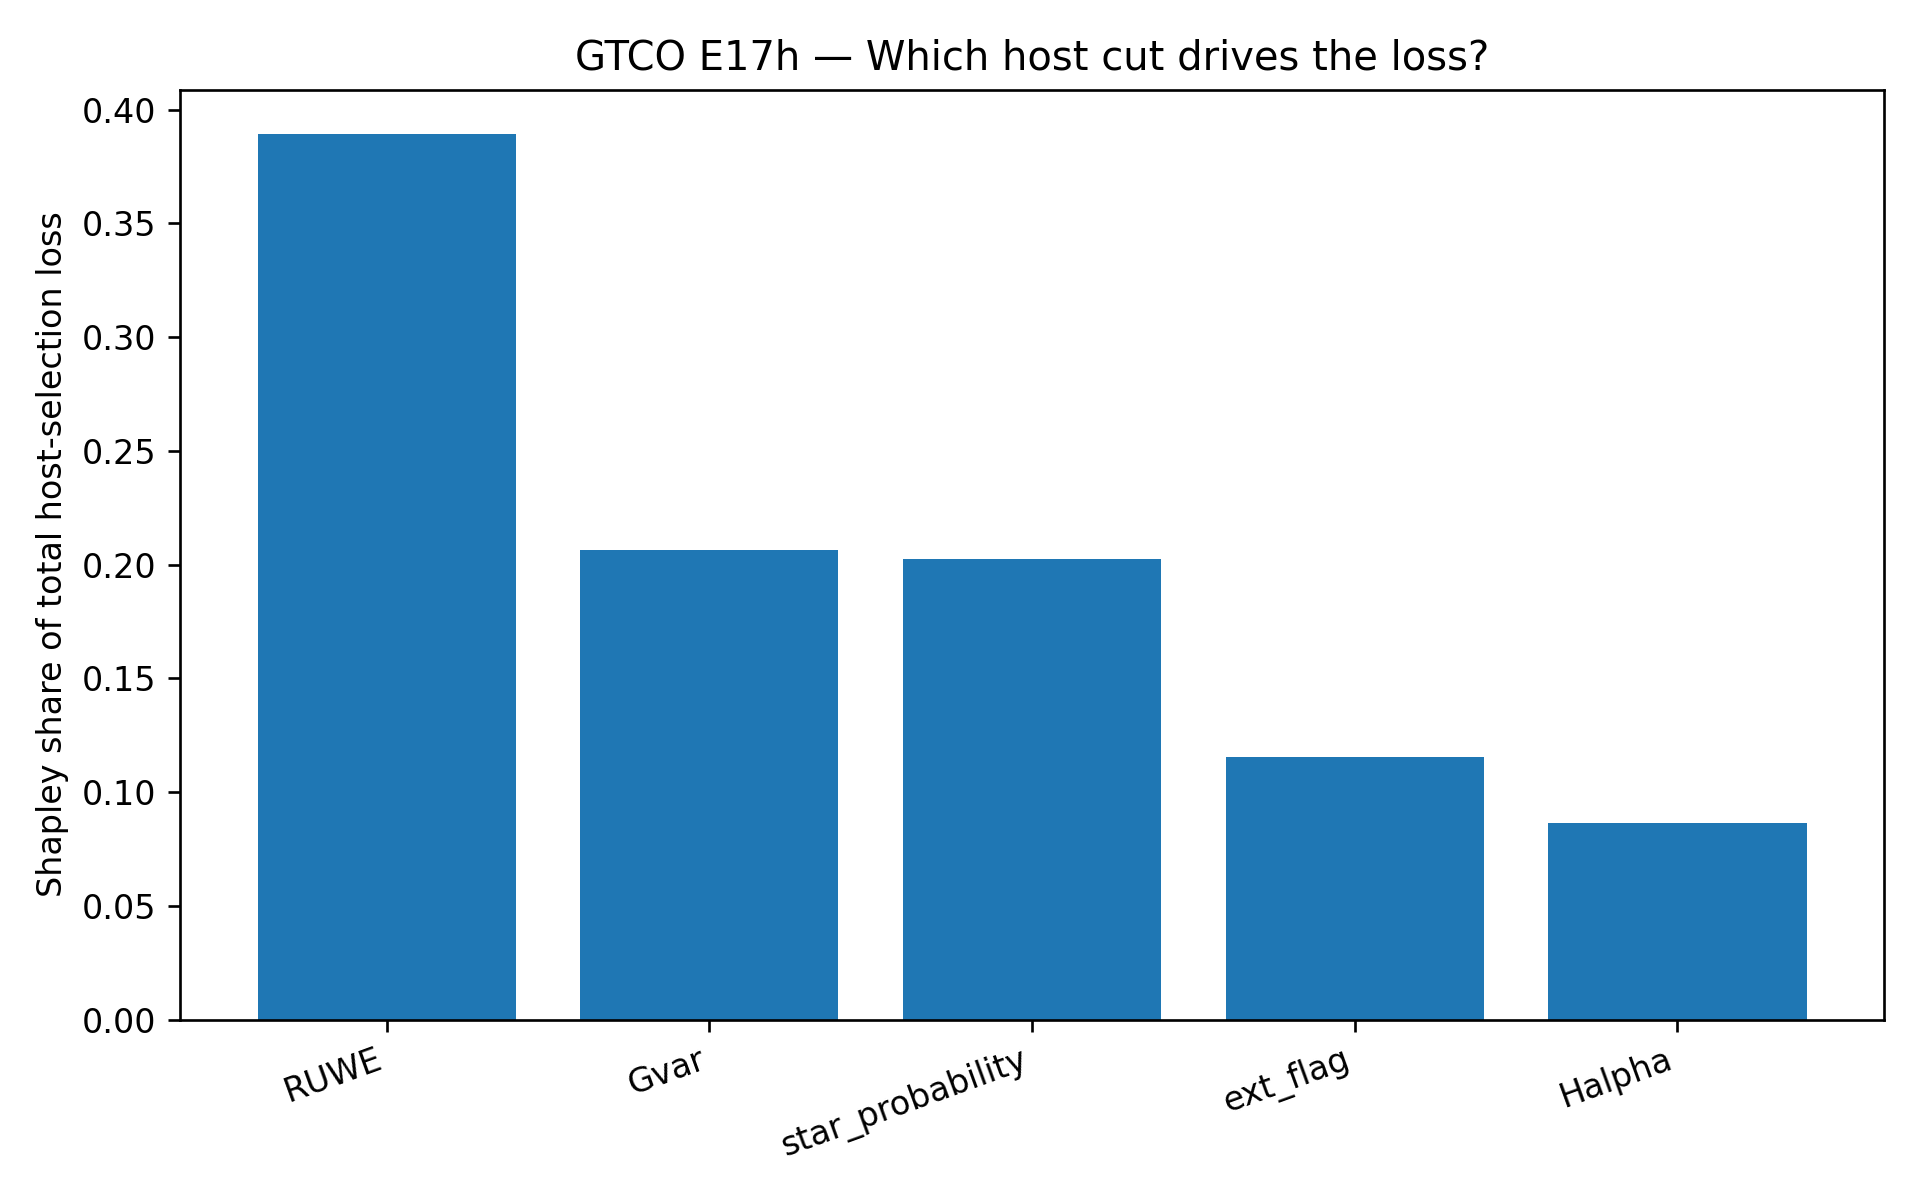
\includegraphics[width=\columnwidth]{figures/fig4_hostcut_shapley.png}
\caption{Shapley attribution of the overlapping \emph{baseline observed} host-gate loss in the 3,000-star validation sample. The value measures how strongly each cut contributes to removal across all cut orderings; it does not evaluate whether the cut should be retained or predict the counterfactual host response of an injected Dyson phenotype.}
\label{fig:shapley}
\end{figure}

\subsection{Source-level coupling of injected photometry and baseline host state}
\label{sec:joint}

A common approximation is to multiply stage-averaged responses,
\begin{equation}
C_{\rm factorized}=\langle C_{\rm phot}\rangle\langle C_{\rm host,base}\rangle.
\end{equation}
That product ignores source dependence. Here the same real stars that are easier or harder to recover photometrically also carry different observed astrometric, classification, variability, and WISE-quality states.

We therefore combine each injected photometric outcome with the \emph{baseline observed} host gate of the same source identity. Averaged over the 54 truth cells,
\begin{equation}
\left\langle C_{\rm phot\cap host,base\mid V}\right\rangle=0.4142,
\end{equation}
whereas the product of stage means gives
\begin{equation}
0.91054\times0.442=0.4025.
\end{equation}
The same-source coupling is 0.0118 higher in absolute terms, or 2.9 per cent relative to the factorized approximation. A 20,000-replicate bootstrap that resamples the 3,000 source identities as clusters gives a 95 per cent interval
\begin{equation}
\Delta C \equiv C_{\rm joint,base}-C_{\rm factorized}
=0.0118\;[0.0089,0.0147].
\end{equation}
Thus the dependence is resolved with respect to host sampling in this frozen validation set. This does \emph{not} convert the baseline host gate into a counterfactual host completeness; it only demonstrates that stage-average multiplication discards real source-level dependence.

\begin{figure}
\centering
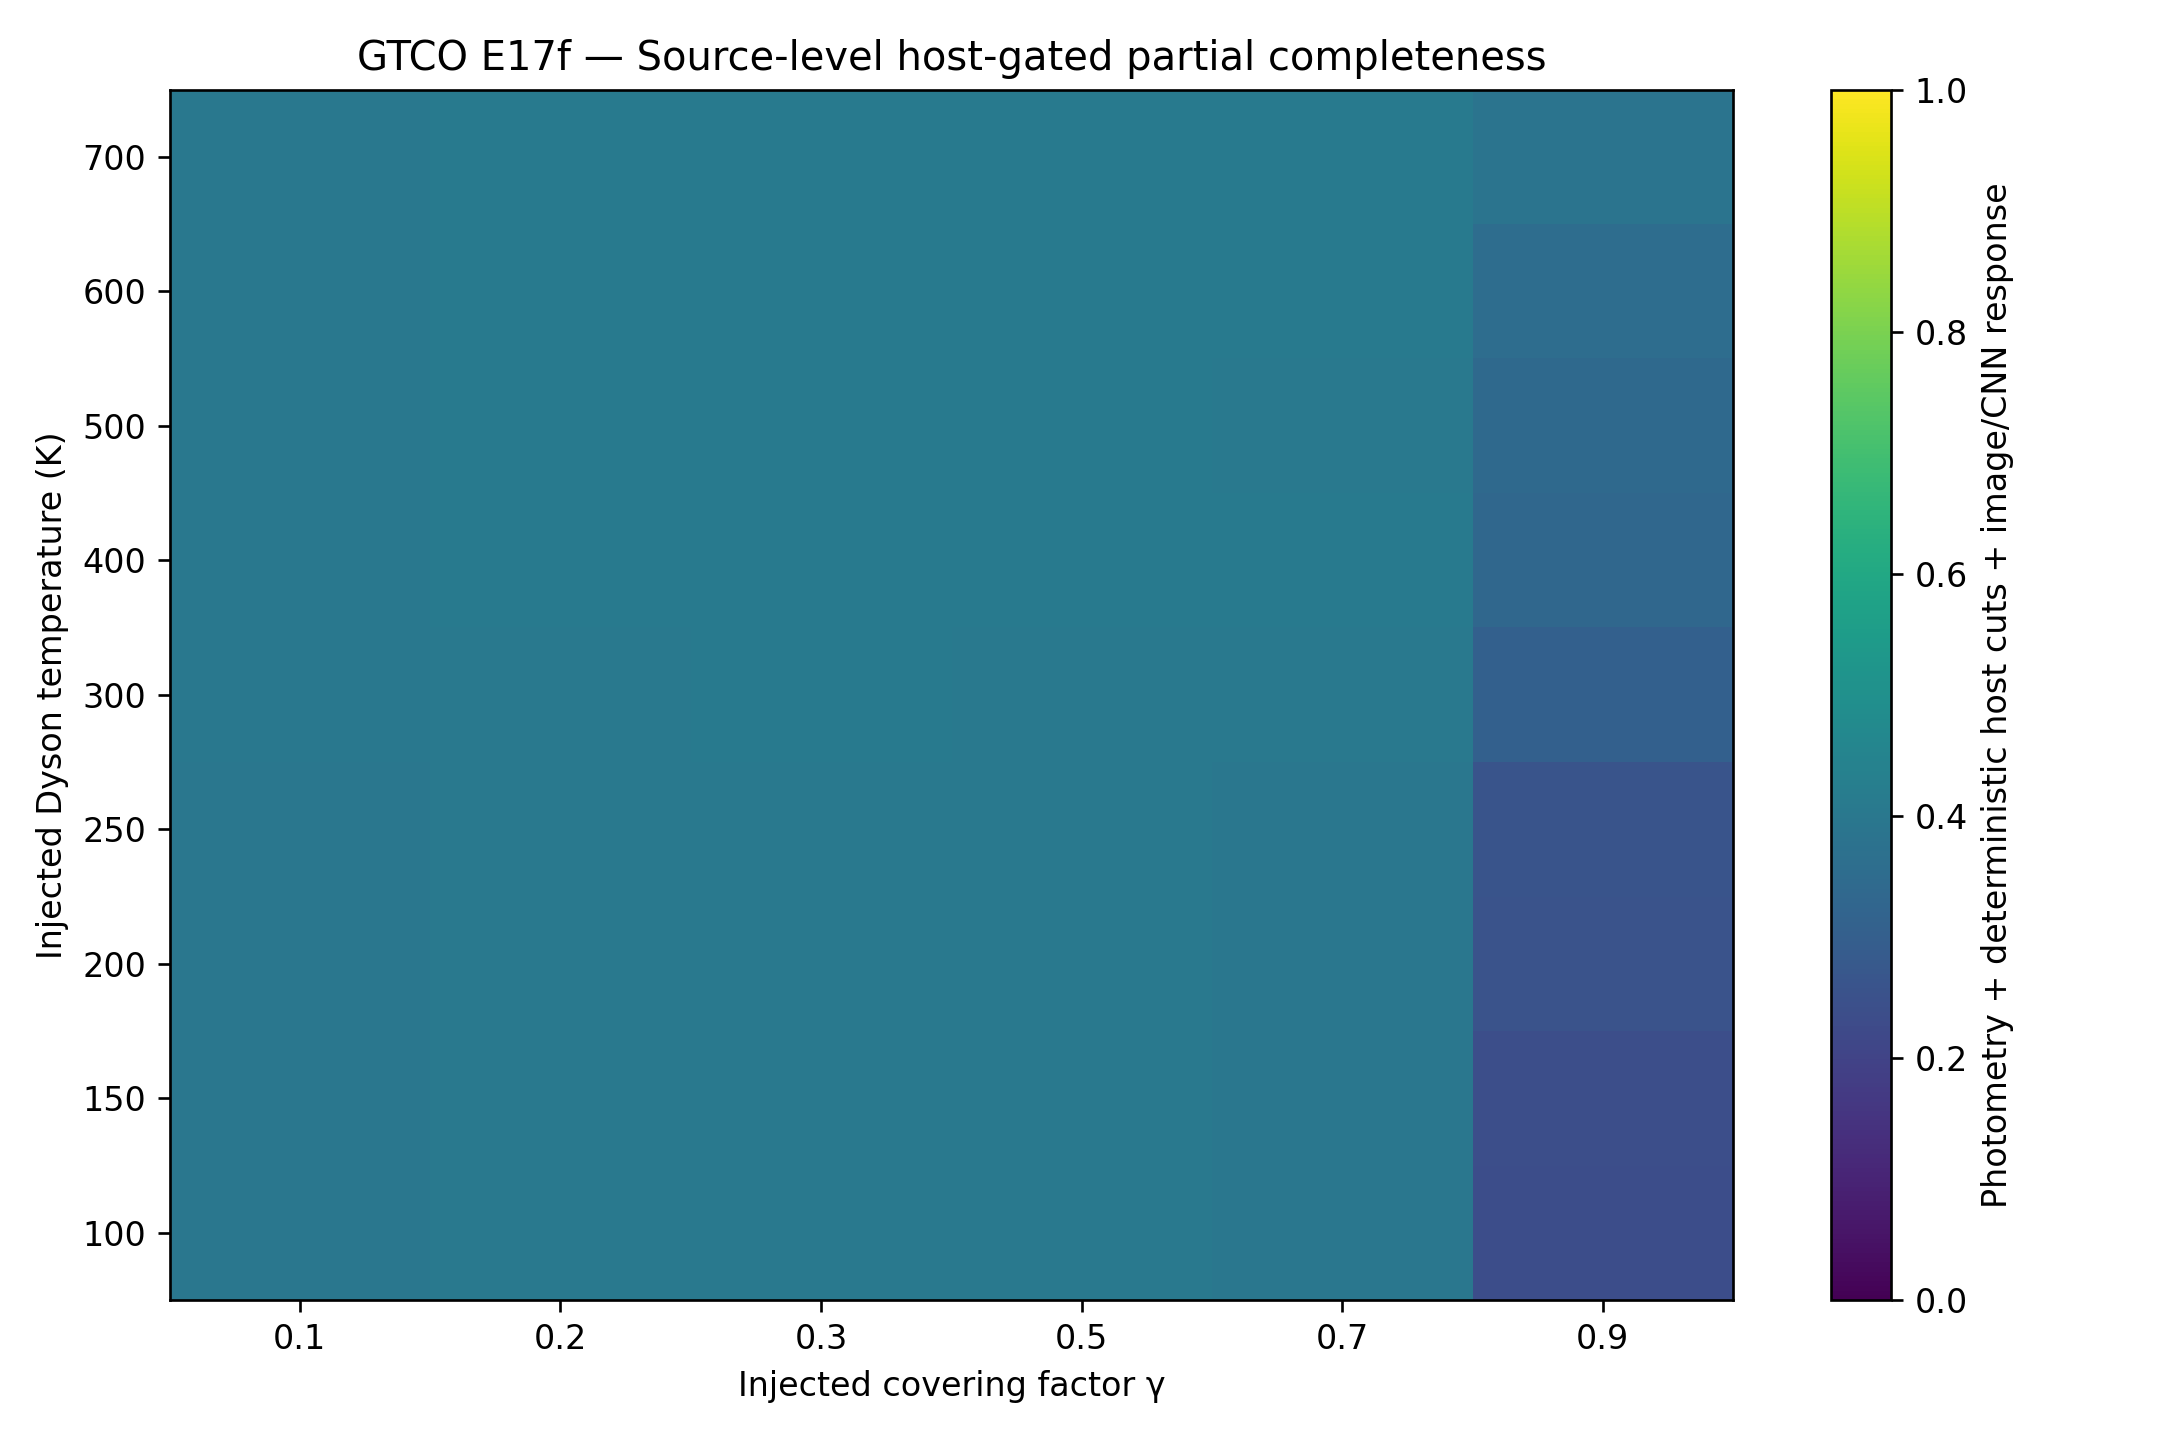
\includegraphics[width=\columnwidth]{figures/fig3_host_gated_completeness.png}
\caption{Same-source coupling between injected photometric recovery and the baseline observed deterministic host gate across the partial-Dyson grid. Each injection is paired with the host-quality state of the same real validation star. The surface is not a full counterfactual host completeness because host catalogue quantities are not regenerated after injection.}
\label{fig:hostsurface}
\end{figure}

The general statistical point remains
\begin{equation}
E[C_1(\mathbf{x})C_2(\mathbf{x})]
\ne
E[C_1(\mathbf{x})]E[C_2(\mathbf{x})]
\end{equation}
when stages share source-property dependence. For end-to-end population inference, the stronger target is a source-level counterfactual forward model for every stage; where that is not available, baseline-state coupling and genuinely counterfactual completeness should be named separately.

\section{Real AllWISE image injection}
\label{sec:image}

\subsection{AllWISE image products}

The image experiment uses 24 bright, low-confusion calibration stars from the 3,000-star validation set. All 24 have AllWISE ${\tt cc\_flags}=0000$, ${\tt ext\_flag}=0$, and Gaia RUWE $<1.4$; 23/24 have zero reported WISE mates and a Gaia--AllWISE catalogue offset below 0.3 arcsec, while one retained boundary case has one reported mate and an offset of 0.446 arcsec. The sample spans W3 $=4.46$--8.48 mag and W4 $=4.41$--7.94 mag. Using $1/(0.4\ln10\,\sigma_m)$ as an approximate magnitude-error signal-to-noise conversion, the median catalogue S/N is 63.9 in W3 and 11.3 in W4. The median central coverage is 17.9 and 19.2 frames, respectively. For each star we retrieved W3 and W4 AllWISE Atlas intensity, uncertainty, and depth-of-coverage cutouts, giving
\begin{equation}
24\times2\times3=144
\end{equation}
FITS products. The AllWISE Atlas has a pixel scale of 1.375 arcsec pixel$^{-1}$ and supplies co-registered intensity, uncertainty, and coverage products in each WISE band \citep{Cutri2013}. These fields are an image-calibration sample, not a representative draw from the full distribution of WISE backgrounds, crowding, and source brightness. This design is deliberate: the experiment asks whether adding a true co-spatial point-source excess to an otherwise acceptable image tends to create a morphology rejection.

The AllWISE documentation notes that resampling and interpolation produce correlated pixel noise in Atlas images \citep{Cutri2013}. Consequently, the uncertainty-weighted residual statistic used below is treated as a \emph{pseudo}-$\chi^2$ morphology feature rather than a formally calibrated independent-pixel goodness-of-fit probability. We test the dependence of our result on this feature explicitly in Section~\ref{sec:image_robustness}.

\subsection{Epoch-consistent source centring}

Gaia astrometric positions are referenced to J2016.0 \citep{Lindegren2021}, whereas W3/W4 AllWISE coadds are dominated by the WISE cryogenic epoch near 2010. We propagate each Gaia position to 2010.5 using its Gaia proper motion before locating the stellar position in the WISE WCS. Across the 24 image-calibration stars, the median 2016.0-to-2010.5 displacement is 0.479 arcsec, the 95th percentile is 1.43 arcsec, and the maximum is 2.81 arcsec. Such shifts are non-negligible compared with the 1.375 arcsec Atlas pixels and would be especially problematic when centroid offset is itself used as a morphology diagnostic. Recent archival analyses of Hephaistos candidates similarly propagate Gaia positions to the WISE epoch before comparing astrometry with mid-infrared centroids \citep{Ren2026}.

\subsection{Empirical PSF and open morphology statistic}

For each band, real source-centred cutouts are background-subtracted in an outer annulus, aligned at sub-pixel precision using their positive central flux, normalized by a central aperture, and combined into an empirical point-source template. The final submission analysis is leave-one-host-out (LOHO): when star $i$ is tested, the empirical PSF is rebuilt from the other 23 stars only.

For a test image, the empirical PSF amplitude is estimated by uncertainty weighting over a central fitting region. The open morphology feature vector contains
\begin{enumerate}
\item the logarithm of an uncertainty-weighted residual pseudo-$\chi^2$;
\item the logarithm of the summed absolute residual normalized by fitted point-source amplitude;
\item the positive-flux centroid offset from the propagated stellar position; and
\item the logarithm of the second-moment major/minor axis ratio.
\end{enumerate}
For each held-out star, the 23 non-test hosts also define the robust feature centre and scale using the median and median absolute deviation. The anomaly score is the maximum robust standardized deviation among the active features. Our default empirical envelope sets the threshold to the maximum score among the 23 training hosts. Thus a held-out baseline image is called clean only if it lies within the entire non-test empirical envelope. This has finite-sample granularity of order one host in 24; it is a transparent open operator, not a reconstruction of the proprietary state of the original Hephaistos image CNN.

\subsection{Co-spatial waste-heat injection and linearity domain}

For each held-out real image, we scan
\begin{equation}
T_{\rm DS}=\{100,150,200,250,300\}\ {\rm K}
\end{equation}
and
\begin{equation}
\gamma=\{0.03,0.05,0.08,0.10,0.14,0.16\},
\end{equation}
producing 720 counterfactuals per band. The physical flux ratio between the baseline catalogued W3/W4 source and the counterfactual follows equation~(\ref{eq:dsmodel}). That ratio is converted to an incremental image amplitude by scaling the fitted point-source amplitude of the real field. The injected image is therefore
\begin{equation}
I_{\rm inj}(x,y)=I_{\rm real}(x,y)+\Delta A\,P_{-i}(x,y),
\end{equation}
where $P_{-i}$ is the empirical PSF constructed without the test host. This formulation preserves the real background, neighbours, coverage, and pixel noise while testing the effect of adding a co-spatial point-like MIR component.

The image operation assumes an approximately linear response. Counterfactuals brighter than the characteristic WISE saturation onsets W3 $=3.8$ mag or W4 $=-0.4$ mag are therefore flagged and excluded from the linear morphology-retention statement \citep{Cutri2012}. Within this deliberately selected 24-star sample and the low-$\gamma$ image grid, 49.7 per cent of W3 counterfactuals and 13.1 per cent of W4 counterfactuals cross those characteristic thresholds. These are not population saturation rates; they are diagnostics of the chosen bright host sample and phenotype grid. WISE can still extract some saturated-source photometry from unsaturated PSF wings, so a full $C_{\rm linear}$ calculation would require explicit bright-source/non-linear forward modelling rather than treating these thresholds as hard catalogue incompleteness.

\section{Real-image results and robustness}
\label{sec:image_results}

\subsection{Matched-operator LOHO diagnostic}

Under the default LOHO construction, the same empirical PSF $P_{-i}$ is used as the injection template and as the reference point-source model for scoring. In W3, 23 of the 24 held-out baseline fields lie within their corresponding LOHO empirical envelope. After excluding saturation-risk counterfactuals, these 23 independent baseline-clean hosts contribute 332 valid injected grid cases and no injection is rejected. The matched-operator W4 calculation likewise has 23 baseline-clean hosts and 596 valid counterfactuals with no rejection.

The repeated $(T_{\rm DS},\gamma)$ grid cells are not independent realizations of the image environment. For W3 we therefore define a host-level success as a host for which all valid injected phenotypes remain accepted. This gives 23/23 successful independent hosts. The one-sided 95 per cent exact binomial lower limit is
\begin{equation}
R_{\rm morph,W3}^{\rm tested}>0.878.
\end{equation}
This confidence statement is retained for W3 because Section~\ref{sec:psf_mismatch} shows that all 23 W3 hosts also remain accepted when the injection PSF is separated from or perturbed relative to the scoring PSF. We do not promote the analogous matched-operator W4 23/23 result to a robust morphology-completeness bound because W4 fails that PSF-mismatch challenge.

\subsection{Metric and threshold ablation}
\label{sec:image_robustness}

The AllWISE Atlas uncertainty map does not encode the full inter-pixel covariance introduced by coaddition, so the pseudo-$\chi^2$ feature should not be essential to the W3 conclusion. We reran the LOHO experiment using four feature sets: the default four-metric score; the same score with pseudo-$\chi^2$ removed; centroid plus axis ratio only; and normalized residual only. We also changed the empirical envelope from the maximum training score to the 95th and 90th percentiles of the 23 training-host scores. Table~\ref{tab:ablation} summarizes the W3 result.

\begin{table}
\centering
\caption{W3 LOHO metric/threshold robustness. $N_{\rm clean}$ is the number of held-out baseline hosts satisfying the specified empirical envelope. Every valid unsaturated injection remains accepted.}
\label{tab:ablation}
\begin{tabular}{llrr}
\toprule
Feature set & Threshold & $N_{\rm clean}$ & Retention\\
\midrule
Four metrics & 90th pct. & 20 & 1.000\\
Four metrics & 95th pct. & 22 & 1.000\\
Four metrics & maximum & 23 & 1.000\\
No pseudo-$\chi^2$ & maximum & 23 & 1.000\\
Centroid + axis ratio & maximum & 23 & 1.000\\
Residual only & maximum & 23 & 1.000\\
\bottomrule
\end{tabular}
\end{table}

Thus the W3 result does not depend on treating the Atlas uncertainty map as an independent-pixel covariance model or on one particular empirical threshold. The matched-operator W4 calculation also passes these feature/threshold ablations, but the stronger challenge is PSF-model mismatch rather than metric choice.

\subsection{Injection/scoring PSF mismatch challenge}
\label{sec:psf_mismatch}

The matched-operator experiment has a structural property: the artificial point-source increment is proportional to the same empirical PSF family used to define the point-source morphology score. LOHO removes test-host leakage but does not, by itself, test sensitivity to a misspecified injection PSF. We therefore repeated the image experiment while keeping the scoring PSF fixed and perturbing only the injection template. The controlled challenges use Gaussian broadening of the empirical template and subpixel offsets of 0.1, 0.25, and 0.5 Atlas pixel; an additional stress test builds injection and scoring PSFs from disjoint subsets of the non-test stars.

The band dependence is strong (Table~\ref{tab:psfmismatch}; Fig.~\ref{fig:psfmismatch}). W3 retains every valid injection in all tested challenges, including the disjoint empirical-PSF split. W4 does not. Its grid-cell retention falls from 1.000 in the matched case to 0.451 under mild broadening and 0.362 for a 0.1-pixel (0.138 arcsec) injection offset; stronger perturbations reduce it further. The disjoint empirical-PSF split gives W4 retention 0.030. Because the 24-star W4 PSF estimate itself is noisy, the disjoint split is intentionally severe; nevertheless, the continuous perturbation sequence shows that the W4 conclusion is already sensitive to much smaller mismatch.

\begin{table}
\centering
\caption{Conditional grid-cell retention under injection-PSF mismatch. The scoring PSF and morphology calibration remain LOHO. Grid cells are repeated phenotypes on the same hosts and are not independent Bernoulli trials. The disjoint-split case is a severe empirical-PSF stress test.}
\label{tab:psfmismatch}
\begin{tabular}{lrr}
\toprule
Challenge & W3 grid-cell & W4 grid-cell\\
\midrule
Matched PSF & 1.000 & 1.000\\
Mild broadening & 1.000 & 0.451\\
Moderate broadening & 1.000 & 0.171\\
0.1-pixel offset & 1.000 & 0.362\\
0.25-pixel offset & 1.000 & 0.136\\
0.5-pixel offset & 1.000 & 0.042\\
Disjoint empirical PSF & 1.000 & 0.030\\
\bottomrule
\end{tabular}
\end{table}

\begin{figure}
\centering
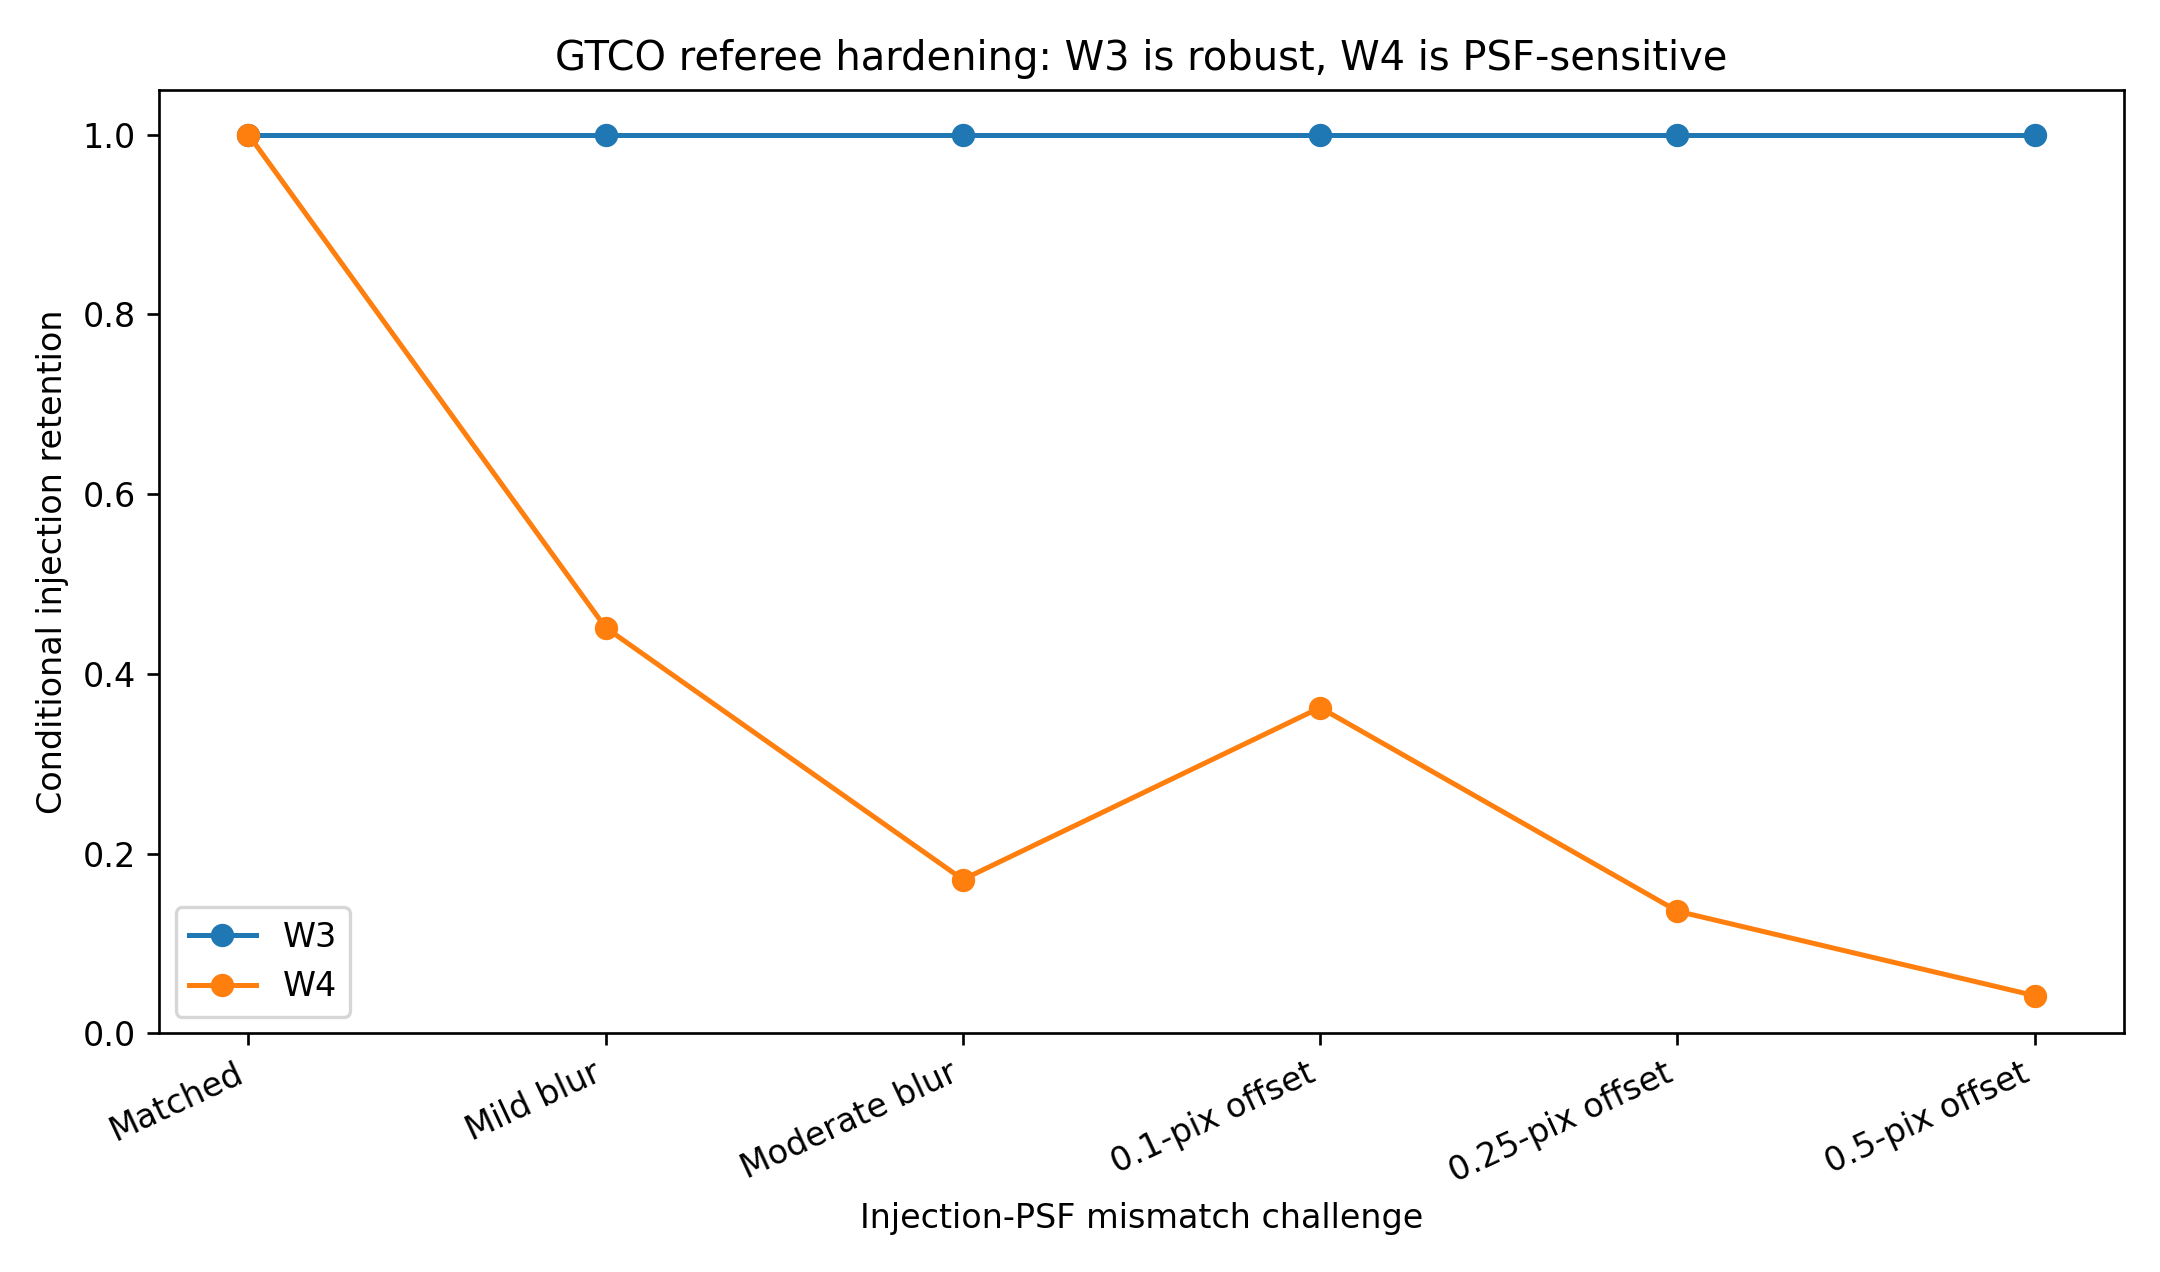
\includegraphics[width=\columnwidth]{figures/fig8_psf_mismatch_robustness.png}
\caption{Conditional image retention when the injection PSF is perturbed while the LOHO scoring PSF is held fixed. W3 is stable across the tested broadening and subpixel-offset challenges; W4 is strongly PSF-model dependent. The disjoint empirical-PSF split is reported in Table~\ref{tab:psfmismatch} but omitted from the continuous-mismatch sequence plotted here.}
\label{fig:psfmismatch}
\end{figure}

The appropriate interpretation is therefore asymmetric. For these 23 clean, unsaturated hosts, co-spatial W3 morphology retention is robust to the tested operator perturbations. The W4 matched-PSF result is an operator-conditional diagnostic, not a robust completeness measurement. This distinction replaces the stronger matched-operator W3/W4 headline used in earlier internal drafts.

\subsection{Image-stage decomposition}

The image-stage response is most safely written as a conditional chain rather than as a product that could be misread as an independence assumption. Let $E$ denote an acceptable baseline environment, $L$ a detector/catalogue regime in which the adopted linearized injection operator is valid, and $M$ morphology acceptance under a specified image operator $\mathcal{O}_{\rm image}$. Then
\begin{equation}
C_{\rm image}
=P(E)\,P(L\mid E)\,P(M\mid E,L,\mathcal{O}_{\rm image}).
\label{eq:image_decomp}
\end{equation}
We refer to these factors heuristically as $C_{\rm environment}$, $C_{\rm linear\mid environment}$, and $R_{\rm morph\mid environment,linear,operator}$, respectively. The present 24-star experiment conditions on deliberately acceptable fields and excludes saturation-risk counterfactuals, so it constrains only the final conditional term for the tested open operator. The W3 tests show that this conditional term is stable to the operator perturbations considered here; W4 demonstrates that the term can itself depend strongly on PSF modelling.

This distinction is observationally consequential. WISE confusion is a known failure mode in ordinary infrared-excess surveys \citep{KennedyWyatt2012}, and the Hephaistos follow-up sequence provides direct examples in which higher angular resolution identifies background galaxies unresolved or blended in WISE \citep{Ren2025,Ren2026,Zackrisson2026}. A future representative field sample should therefore target $P(E)$, while W4 additionally requires a better-constrained source-specific PSF/operator model before a morphology response can be assigned a stable scalar value.

\section{From candidates to population constraints}
\label{sec:population}

Equation~(\ref{eq:selection_inversion}) becomes useful only after every factor has a matched operational definition. The seven final candidates reported by \citet{Suazo2024}, for example, provide a final-candidate rate for the published Hephaistos-II decision chain. Our 0.910 photometric response is not the completeness of that seven-candidate operator: it does not reproduce the original CNN weights, the full image-confusion decision, every downstream astrophysical cut, or the final manual review. Dividing the published final-candidate rate by 0.910 would therefore combine incompatible selection definitions.

Likewise, $C_{\rm DS}$ is not a universal scalar. Let $\boldsymbol\psi$ denote technosignature phenotype parameters such as $(T_{\rm DS},\gamma)$ and let $\mathbf{x}$ denote host and observing conditions. A population-averaged completeness is
\begin{equation}
\bar C_{\rm DS}=
\int C_{\rm DS}(\boldsymbol\psi,\mathbf{x})
\,p(\boldsymbol\psi,\mathbf{x}\mid{\rm DS})
\,{\rm d}\boldsymbol\psi\,{\rm d}\mathbf{x}.
\label{eq:marginal_completeness}
\end{equation}
The numerical value therefore depends on a declared phenotype distribution, or else should be reported as a response surface rather than compressed into one number. This is why the arithmetic mean of 0.910 over our 54 equally weighted truth cells is useful as an experiment summary but should not be inserted uncritically into an occurrence estimate.

The same logic applies to candidate composition. $\pi_{\rm DS}$ is the fraction of objects admitted by the candidate operator that genuinely belong to the target phenotype. It is not obtained by normalizing a discriminative SED score unless that score has been calibrated as a likelihood for the selected population. High-resolution follow-up changes what is known about individual candidates and, with an explicitly modelled follow-up selection, can improve inference on candidate composition; it does not retroactively convert an unmatched upstream completeness into a final-pipeline response.

The immediate population-inference target is therefore a selection-consistent chain in which the parent definition, candidate definition, signal injection, image/environment response, and follow-up interpretation are frozen together. The current work calibrates several of those pieces and, equally importantly, identifies the unmeasured terms instead of absorbing them into an apparently precise scalar.

\section{Discussion}

\subsection{Relationship to astronomical selection-function work}

The principal statistical ideas used here are not unique to technosignature searches. Survey selection functions have long been recognized as essential for inferring population properties from non-random astronomical samples \citep{EverallDas2020,BoubertEverall2022}. Our contribution is to operationalize that logic for a multi-stage partial-Dyson search in which the signal phenotype can be injected into real stellar measurements. The distinction between a catalogue-level subset selection and an intrinsic population selection is especially relevant: a deterministic cut on reported quantities is a binary decision for a fixed catalogue row, but the probability of a real or counterfactual astrophysical source satisfying that cut requires propagation through measurement uncertainty and catalogue construction \citep{BoubertEverall2022}.

This perspective also changes how a quality cut should be discussed. The fact that RUWE supplies the largest Shapley contribution to our reconstructed host loss does not imply that RUWE $<1.4$ is a poor cut. Gaia subset selection functions with precisely this RUWE threshold are known to vary with magnitude, colour, and sky position \citep{EverallBoubert2022}. The scientific question is therefore not simply whether the cut removes many objects, but whether $P({\rm RUWE}<1.4\mid{\rm true\ phenotype},\mathbf{x})$ is calibrated for the population being constrained.

\subsection{Why image environment, signal morphology, and PSF modelling are different problems}

The real-image experiment separates three issues that can be blurred when image screening is represented by one efficiency. First, a WISE field can fail because it contains an offset red galaxy, a blend, structured background, an artefact, or a resolved/extended source. Those are environment and survey-resolution effects. Secondly, a genuinely co-spatial unresolved waste-heat component changes the central point-source flux rather than introducing a new offset object. Thirdly, any quantitative morphology decision depends on how accurately the image operator models the band-specific PSF.

The W3 results support the geometric expectation over the tested range: the 23 clean, unsaturated hosts survive not only the matched-PSF LOHO injection but also threshold/feature ablations, independent empirical-PSF splits, moderate PSF broadening, and subpixel offsets. W4 is an important counterexample to over-generalization. Its matched-PSF experiment also gives 23/23 host successes, but small PSF perturbations cause substantial losses. Thus ``co-spatial point source'' is not by itself sufficient to guarantee a stable image-selection response when the scoring operator is PSF-sensitive.

This does not make image screening unimportant; it makes the scientific targets more precise. Recent Hephaistos follow-up results show that environmental confusion is where high-resolution information is valuable \citep{Ren2025,Ren2026,Zackrisson2026}. A representative $P(E)$ calibration should stratify by WISE neighbour count, astrometric offset, local background, coverage, and Galactic latitude. In parallel, a W4 morphology calibration should use a better-constrained local or source-specific PSF model rather than extrapolating the matched empirical-template result into a survey-wide completeness claim.

\subsection{Implications for previous and future occurrence limits}

Hephaistos-I reports upper limits as functions of Dyson temperature, covering fraction, and distance, explicitly recognizing that lower covering fractions are more easily confused with natural infrared emission and that WISE sensitivity weakens with distance \citep{Suazo2022}. Our results are complementary rather than a re-analysis of those published limits. We focus on the response semantics of a candidate pipeline and on source-level coupling between stages. The present analysis does not invalidate earlier phenotype-conditioned upper limits; it shows why a later, more elaborate final-candidate operator requires its own matched completeness if the candidate count is to be inverted into an occurrence estimate.

The practical design principle is therefore to freeze the candidate operator before occurrence inference and inject the target phenotype through that operator at the finest feasible level. Where exact stages are unavailable---for example, an unpublished historical CNN state or a manual visual decision---their response should remain an explicit uncertainty or be replaced by a newly defined reproducible operator, rather than silently approximated by an unrelated upstream efficiency.

\subsection{Limitations and external validity}
\label{sec:limitations}

Several limitations define the claim boundary.

First, the parent catalogue used here is a nominal 100-pc Gaia sample, whereas Hephaistos-II searched a larger sample out to 300 pc \citep{Suazo2024}. The distance distribution, WISE sensitivity, crowding, and background environment are therefore not matched to the published final-candidate sample.

Secondly, the photometric experiment is a close emulation rather than a code reproduction. The exact identities of the original 265 Hephaistos-II templates, exact internal grid spacing if non-uniform, full response-curve synthetic photometry, and all intermediate pipeline state are not available in the executable operator used here. The saturation audit further shows that our frozen 265-star library is not identical to the published template-selection semantics in W1/W2. Correction-aware sensitivity tests leave the mean response near 0.91--0.92, while a literal four-band onset-threshold hard cut destroys the bright end of the stated template coverage and is therefore retained only as a stress test.

Thirdly, the baseline injection uses each source's measured catalogue uncertainty as the default absolute noise scale. A conservative flux-dependent floor-plus-Poisson bracket leaves the mean response essentially unchanged (0.910309 versus 0.910537), but more extreme prescriptions span a wider range. A full survey forward model would propagate band-specific measurement, background, calibration, and saturation behaviour as functions of counterfactual flux.

Fourthly, the 3,000-star validation set is conditional on complete baseline ten-band photometry and uncertainty information. The 0.910 response therefore does not include the probability that an arbitrary CMD-selected parent star enters this validation-eligible pool. Section~\ref{sec:conditioning} exposes this conditioning instead of folding analysis-supporting availability into a final candidate completeness.

Fifthly, the deterministic host quantity is the observed \emph{baseline} host state of the validation sources. It is not $P({\rm host\ pass}\mid{\rm injected\ DS})$. A large covering factor can alter Gaia brightness and hence the distribution or availability of classification, variability, and quality products. The 0.414 result is consequently a same-source coupling diagnostic, not a counterfactual host completeness. The exact numerical neighbourhood used in the original $G_{\rm var}$ normalization is also not public; the 500--5,000-source sensitivity test shows that this narrower implementation ambiguity is small.

Sixthly, the image experiment contains only 24 deliberately clean fields. It does not estimate the probability that a random WISE environment is unconfused, and the original Hephaistos CNN and final visual operator are not reproduced. The W3 result is robust to the tested PSF perturbations, but W4 is not: its matched-operator retention is highly sensitive to modest injection/scoring PSF mismatch. The W4 result is therefore retained as an operator-sensitivity finding rather than a completeness bound.

Seventhly, the real-image injection is interpreted only outside characteristic WISE saturation thresholds. Saturated counterfactuals are flagged, not propagated through a detector/non-linear image model. The AllWISE Atlas also contains correlated pixel noise; this is why the residual $\chi^2$ is treated as a pseudo-statistic and why feature ablation is part of the submission analysis.

Finally, the single-temperature blackbody phenotype in equation~(\ref{eq:dsmodel}) is deliberately restricted. More complex waste-heat spectra, anisotropy, non-grey obscuration, or technosignatures not dominated by mid-infrared waste heat can have different selection functions. A non-detection constrains the searched phenotype, not technological civilizations in general.

These limitations are the reason no stellar Dyson-sphere occurrence rate is quoted here. The analysis is intended to make the path to such an inference more auditable, not to create a numerically strong constraint by combining unmatched response terms.

\section{Reproducibility and audit trail}
\label{sec:repro}

The submission-critical analysis is separated from the earlier exploratory research history. Frozen inputs are recorded by filename, byte size, and SHA-256 hash. The 24-star real-image analysis has a per-product manifest covering all 144 W3/W4 intensity, uncertainty, and coverage FITS files. The public reproduction path contains separate scripts for input verification, deterministic baseline host cuts, standalone E12c/E17f photometric--host reconstruction, LOHO real-image injection, host-level confidence intervals, metric/threshold ablation, photometric noise bracketing, injection/scoring PSF-mismatch challenges, WISE blackbody colour-correction/isophotal-wavelength sensitivity, and the all-band-unsaturated validation-subset check. The standalone catalogue reconstruction rebuilds the 220,745-model library from the frozen real templates and reruns all 54 truth cells on the 3,000 validation stars rather than reading frozen summary tables as inputs. Alternative correction-aware template tables, the four-band hard-cut stress-test table, source-cluster bootstrap results, colour-correction outputs, validation-conditioning outputs, and PSF-mismatch case summaries are frozen alongside the manuscript outputs.

The numerical workflow uses Python with NumPy, pandas, SciPy, and Matplotlib \citep{Harris2020,McKinney2010,Virtanen2020,Hunter2007}. The repository also contains frozen result tables, claim boundaries distinguishing supported and unsupported interpretations, and a manuscript copy. Rejected or exploratory calculations are not silently promoted into the submission path. In particular, the independent host rather than the repeated injection grid cell is used as the statistical unit for the final real-image confidence statement.

At the time of this draft the public code repository is
\begin{center}
\url{https://github.com/Wujijiandao/gtco-dyson-selection-calibration}.
\end{center}
A versioned archival DOI will be inserted in the final submission after the corresponding GitHub release is deposited in Zenodo.

\section{Conclusions}

We have developed and audited a selection-calibration framework for mid-infrared partial-Dyson searches based on Gaia DR3, 2MASS, and AllWISE data. The main results are:

\begin{enumerate}
\item A 220,745-model, real-star injection--recovery experiment gives a mean conditional SED-recognition response of approximately 0.910 over the tested 54-cell $(T_{\rm DS},\gamma)$ grid. The standalone executable reconstruction gives 0.910537 versus the frozen 0.910543. A conservative floor-plus-Poisson flux-noise bracket gives 0.910309, W2-correction-aware template tests give 0.911--0.917, and a WISE blackbody colour-correction/isophotal-wavelength sensitivity gives 0.911568. Thus the 0.91 summary is stable to the reasonable hardening variants tested here, although it remains conditional on the validation-eligible ten-band sample and on the adopted SED emulation.

\item The observed baseline Gaia/WISE host gate passes 0.442 of the same 3,000 validation stars. Combining each injected photometric outcome with the baseline host state of the same source gives 0.414, whereas multiplying stage means gives 0.402. The difference is $0.0118$ with a 95 per cent source-cluster bootstrap interval of $0.0089$--$0.0147$. This demonstrates measurable same-source dependence, but 0.414 is not a counterfactual host completeness because Gaia/WISE host products are not regenerated after injection.

\item In real AllWISE W3 images, LOHO co-spatial injection produces no morphology failure among 23 independent baseline-clean, unsaturated hosts. W3 remains fully retained after removing the pseudo-$\chi^2$ feature, changing empirical thresholds, splitting the empirical injection/scoring PSFs, moderate PSF broadening, and offsets up to 0.5 Atlas pixel. The one-sided 95 per cent host-level lower bound for the tested W3 response is 0.878.

\item W4 does not support the same robust scalar statement. Its matched-PSF LOHO grid-cell retention is 1.000, but grid-cell retention falls to 0.451 under mild PSF broadening and 0.362 for a 0.1-pixel injection offset, with stronger mismatch producing still lower values. The W4 result is therefore evidence of PSF-model sensitivity rather than a morphology-completeness bound.

\item Image-stage completeness should be represented as a conditional chain,
\begin{equation}
C_{\rm image}=P(E)P(L\mid E)P(M\mid E,L,\mathcal{O}_{\rm image}),
\end{equation}
rather than as interchangeable stage-average efficiencies. The present experiment conditions on clean environments and an unsaturated linearized regime; representative field-environment response remains unmeasured.

\item Candidate rates can be transformed into population occurrence only through a selection-consistent relation,
\begin{equation}
f_{\rm DS}=\pi_{\rm DS}r_{\rm cand}/C_{\rm DS},
\end{equation}
with every quantity defined for the same parent population, phenotype, and candidate operator.
\end{enumerate}

The next empirical priorities are a representative real-image environment calibration, a source-specific W4 PSF/operator calibration, explicit treatment of bright-source non-linearity, and counterfactual modelling of host-quality products. These measurements address the largest remaining response terms without conflating them with the response components already tested here.

\section*{Acknowledgements}

This work makes use of data from the ESA \textit{Gaia} mission, 2MASS, and the Wide-field Infrared Survey Explorer/AllWISE archive.

\textbf{AI-use disclosure:} OpenAI ChatGPT was used as an interactive research assistant for code prototyping, numerical-analysis workflow development, manuscript drafting, and language editing. The author reviewed the input data, executable analysis steps, numerical outputs, references, and final scientific claims and takes responsibility for the submitted work.

\section*{Data Availability}

The public survey data used in this work are available from the Gaia Archive and the NASA/IPAC Infrared Science Archive. Submission-critical analysis scripts, input hashes, frozen result tables, figure products, and claim-boundary documentation are publicly available at \url{https://github.com/Wujijiandao/gtco-dyson-selection-calibration}. A permanent Zenodo DOI for the frozen submission release will be inserted before final submission. The real AllWISE cutouts used for the 24-field image-response experiment can be regenerated from source coordinates and the per-file IRSA product manifest supplied in the repository.

\bibliographystyle{mnras}
\bibliography{references}

\appendix

\section{Frozen selection semantics}
\label{app:semantics}

For reproducibility, the deterministic host semantics are summarized here. H$\alpha$ emission is considered significant only if both equivalent width and its uncertainty are available and $EW+3\sigma<0$; otherwise the H$\alpha$ cut passes. RUWE must be non-missing and $\le1.4$. AllWISE ${\tt ext\_flag}$ must be non-missing and equal to zero. Gaia DSC single-star probability must be non-missing and $>0.9$. $G_{\rm var}$ requires valid $G$ observation count and positive flux-over-error and must be $\le2$. The default local-median reference uses 1,000 magnitude-sorted neighbouring sources, with 500 and 5,000 used as sensitivity checks.

For the photometric validation experiment, the 265 template stars and the 3,000 validation stars are disjoint. Both are drawn from the strict ten-band analysis-supporting pool. The truth grid is fixed before recovery evaluation, and the default validation noise is source-specific. The frozen random seed used for the reconstructed validation injection is recorded in the reproduction materials. Alternative W2-corrected template tables, a literal saturation-onset stress-test table, and flux-dependent noise brackets are stored as sensitivity products rather than silently substituted into the baseline run.

The deterministic host gate is evaluated on the observed baseline catalogue row and is not relabelled as a counterfactual host completeness. For the image experiment, the tested star is excluded from both PSF construction and morphology calibration. Proper motion is propagated from Gaia epoch 2016.0 to a common WISE epoch approximation of 2010.5. The W3/W4 signal is injected at that propagated stellar position. Counterfactuals crossing the characteristic WISE saturation onsets are labelled saturation-risk and excluded from the linear morphology-retention statement. PSF-mismatch challenges keep the scoring operator fixed while modifying the injection template.

\label{lastpage}
\end{document}
